\documentclass{article}
\usepackage{microtype,graphicx,booktabs,tabularx,multirow}
\usepackage{amsmath,amssymb}
\usepackage{tikz}
\usetikzlibrary{arrows.meta,positioning,fit,calc}
\usepackage{hyperref}
\usepackage[preprint]{icml2026}
\icmltitlerunning{Humaneness Ears: Joint Speech Attribute and Vocal Event Prediction}
\newcommand{\he}{\textsc{Humaneness Ears}}
\newcommand{\pthree}{\textsc{P3}}
\newcommand{\nmae}{\mathrm{nMAE}}
\begin{document}
\twocolumn[
\icmltitle{Humaneness Ears: Joint Prediction of Emotion, Voice Style, Audio Quality, Speaker Representations, and Vocal Events}
\begin{icmlauthorlist}\icmlauthor{Anonymous Authors}{anon}\end{icmlauthorlist}
\icmlaffiliation{anon}{Anonymous institution}
\icmlcorrespondingauthor{Anonymous Author}{anon.email@domain.com}
\icmlkeywords{speech understanding, multitask learning, emotion recognition, sound event localization}
\vskip 0.3in
]
\printAffiliationsAndNotice{}

\begin{abstract}
Large audio collections need dense, temporally grounded annotations, yet emotion, delivery, quality, speaker characteristics, and non-speech vocal events are commonly predicted by separate systems. We present \he, two encoder-only Whisper students that jointly output 192 scalar attributes, a speech-rate proxy, two speaker-characteristic embeddings, and frame- and event-level vocal-burst predictions from audio of at most 30 seconds. A layer-aware shared architecture is trained on a nested ten-stage speech curriculum mixed with synthetic event insertions, then adapted for two epochs to a 194-hour pool with Gemini event and attribute annotations and cached specialist-teacher targets. On 3,544 held-out annotation clips, the Base and Medium models obtain timbre cosine similarity of 0.904/0.922 and burst-frame F1 of 0.693/0.689; end-to-end event F1 at intersection-over-union 0.5 is only 0.194/0.195. We also evaluate expert-rated EmoNet-Voice and VoiceNet tasks, acted-emotion corpora, and an independent burst-mixture stress test, identifying substantial domain and localization gaps. These results establish a practical compact joint annotator while clearly separating teacher imitation from human agreement.
\end{abstract}

\section{Introduction}
Web speech clips carry more than words: perceived emotion, delivery, recording quality, speaker characteristics, laughter and other vocal events may all matter for search, data selection, and analysis. Running a separate specialist for every dimension scales inference cost and complicates alignment between clip-level attributes and timed events. \he\ addresses this annotation problem with one trainable acoustic encoder and a family of simultaneous readouts. Its output is deliberately heterogeneous: intensities and quality scores are continuous, speaker representations are vectors, and vocal bursts require both occupancy and interval boundaries.

The contribution is an \emph{integrated student and evaluation}, rather than a claim that any one score constitutes a human judgment. We (i) combine 192 scalar targets, two distinct Orange embedding spaces, literal characters per second (CPS), and 53 vocal-event types with a temporal proposal head; (ii) use pooled features from every Whisper layer and event-local features for classification; and (iii) evaluate teacher imitation, human-label transfer, and localization separately. The study exposes a useful failure mode: after Gemini adaptation, event performance on the earlier synthetic mixture distribution falls, while agreement with the new held-out annotations remains measurable. This distinction is central to the intended use in large-scale annotation.

\section{Related Work}
Whisper supplies multilingual audio representations learned through weakly supervised speech recognition \citep{radford2023whisper}. We retain its encoder but remove the decoder and transcription objective; the resulting model cannot produce words. WavLM similarly motivates treating speech representations as useful for speaker and paralinguistic tasks \citep{chen2022wavlm}. \citet{schuhmann2025emonetface} introduced a fine-grained 40-emotion taxonomy in the visual domain; \citet{schuhmann2025emonetvoice} transferred it to speech with expert-rated synthetic audio and Empathic Insight Voice baselines. \citet{schuhmann2026voicenet} extends evaluation to real-speech emotion and 57 perceptual voice dimensions using audio--text contrastive VoiceCLAP models. \he\ predicts fixed numeric attributes rather than text--audio similarity, so identical benchmark labels need a specified score adapter.

Audio quality is also multidimensional. Audiobox Aesthetics distinguishes content enjoyment/usefulness from production complexity/quality \citep{tjandra2025audiobox}; DNSMOS predicts speech, background, and overall quality proxies \citep{reddy2021dnsmos}. Our model distills outputs of these systems rather than replacing their underlying human-rating studies. For vocal events, our interval task is related to the Whisper-based Vocalburst Locator \citep{laion2026locator}; combining sound-event segmentation with broad paralinguistic outputs is the operational motivation. Speaker targets are the distinct timbre and identity spaces supplied by Orange WavLM models \citep{orange2026timbre,orange2026identity}, not person IDs.

\begin{figure*}[t]
\centering\resizebox{0.98\textwidth}{!}{%
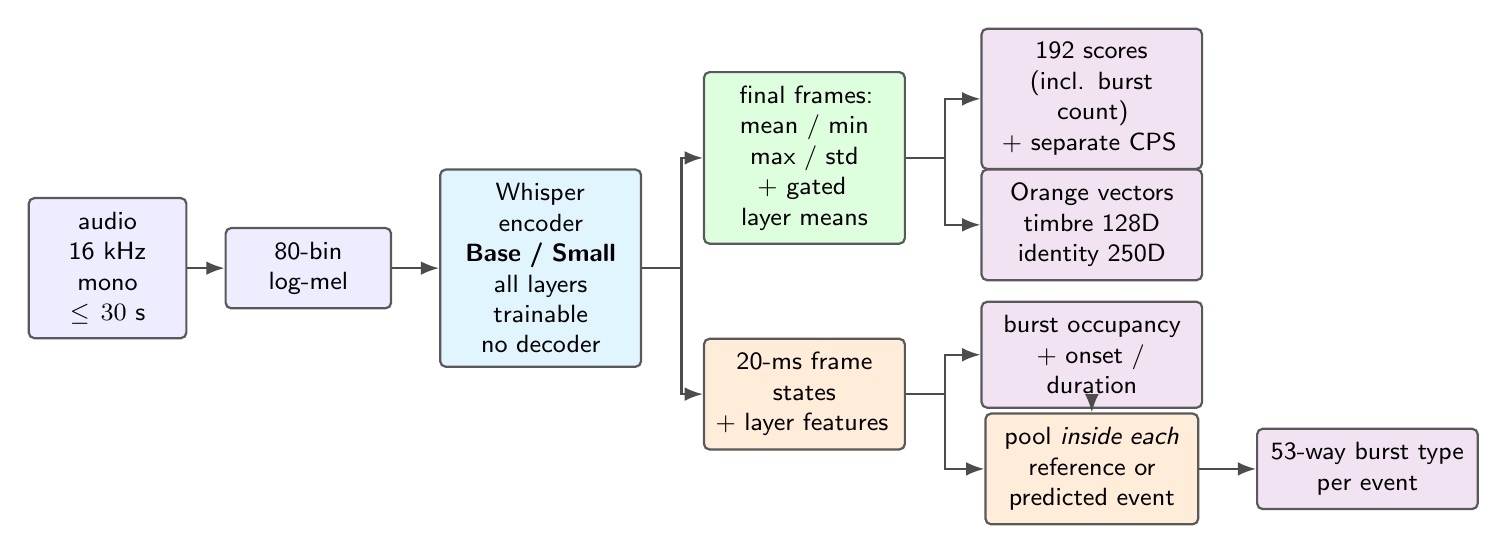
\begin{tikzpicture}[
  >=Latex, font=\sffamily\small,
  box/.style={draw=black!65,rounded corners=2pt,thick,minimum height=1.0cm,align=center,inner sep=5pt},
  source/.style={box,fill=blue!7},
  shared/.style={box,fill=cyan!12},
  global/.style={box,fill=green!13},
  temporal/.style={box,fill=orange!15},
  target/.style={box,fill=violet!11},
  arr/.style={->,thick,draw=black!70}
]
\node[source,text width=1.65cm] (audio) at (0,1.1) {audio\\16 kHz mono\\$\leq30$ s};
\node[source,text width=1.75cm] (mel) at (2.55,1.1) {80-bin\\log-mel};
\node[shared,text width=2.20cm,minimum height=2.1cm] (encoder) at (5.5,1.1) {Whisper encoder\\\textbf{Base / Small}\\all layers trainable\\no decoder};
\node[global,text width=2.20cm] (pool) at (8.85,2.5) {final frames:\\mean / min\\max / std\\+ gated layer means};
\node[temporal,text width=2.20cm] (frames) at (8.85,-0.5) {20-ms frame states\\+ layer features};
\node[target,text width=2.45cm] (scalars) at (12.5,3.25) {192 scores\\(incl. burst count)\\+ separate CPS};
\node[target,text width=2.45cm] (speaker) at (12.5,1.65) {Orange vectors\\timbre 128D\\identity 250D};
\node[target,text width=2.45cm] (occupancy) at (12.5,0.0) {burst occupancy\\+ onset / duration};
\node[temporal,text width=2.35cm] (local) at (12.5,-1.45) {pool \emph{inside each}\\reference or predicted event};
\node[target,text width=2.45cm] (classes) at (16.0,-1.45) {53-way burst type\\per event};
\draw[arr] (audio)--(mel);
\draw[arr] (mel)--(encoder);
\draw[arr] (encoder.east) -- ++(.5,0) |- (pool.west);
\draw[arr] (encoder.east) -- ++(.5,0) |- (frames.west);
\draw[arr] (pool.east) -- ++(.5,0) |- (scalars.west);
\draw[arr] (pool.east) -- ++(.5,0) |- (speaker.west);
\draw[arr] (frames.east) -- ++(.5,0) |- (occupancy.west);
\draw[arr] (frames.east) -- ++(.5,0) |- (local.west);
\draw[arr] (occupancy.south) -- (local.north);
\draw[arr] (local)--(classes);
\end{tikzpicture}%
}

\caption{\he\ uses the pretrained Whisper audio encoder only. Final-frame statistics and gated means of all hidden layers support clip-level tasks. A 20-ms temporal branch predicts occupancy and independent onset/duration proposals; each event class is computed from frames inside that event. Training uses masks for unavailable or inapplicable teacher labels. No ASR decoder, transcript input, or external teacher is used at inference.}
\label{fig:architecture}
\end{figure*}

\section{Model and Objectives}
\paragraph{Input and shared representation.}
Mono 16-kHz audio (0.1--30 s) is converted to 80-bin log-mel features and passed through all layers of a fully trainable Whisper encoder. Base has six layers, width 512, 20.59M encoder parameters; Medium uses the Whisper Small encoder with 12 layers, width 768, 88.15M encoder parameters. With heads, they have 26.44M and 97.10M parameters. The last-layer time sequence yields masked mean, minimum, maximum, and standard deviation, concatenated as the principal clip representation. Each hidden layer also yields a masked time mean. Per-task-family projections of these means (32 or 64 dimensions, 128 for speaker routes) are combined with a sample-dependent softmax gate and added as residual information to the clip heads.

\paragraph{Output heads.}
The 192 scalar slots are 40 EmoNet emotions, 57 VoiceNet dimensions, genuineness, burst blend and a legacy quality slot (three), 19 Empathic Insight extras, four Audiobox axes, seven DNSMOS outputs, 61 VoiceCLAP attributes, and a log-transformed event count. CPS is a separate scalar, defined from Unicode transcript characters including spaces and punctuation divided by full clip duration. Orange timbre (128D) and identity (250D) are separate unit-vector heads. The temporal branch predicts 20-ms burst occupancy, onset logits, and log durations. Independent proposals can overlap, unlike connected regions of the binary mask. A 53-way event classifier pools the final encoder state and the layer mixture \emph{only inside a supplied or predicted interval}; during training it uses reference spans. Figure~\ref{fig:architecture} summarizes the paths.

\paragraph{Masked multitask loss.}
For scalar group $g$, with target-standardized prediction $\hat z_{ij}$, label $z_{ij}$, availability mask $m_{ij}$, and Huber penalty $\rho_1$, the term is
\begin{equation}
\mathcal L_g=\lambda_g\frac{\sum_{i,j\in g}m_{ij}\rho_1(\hat z_{ij}-z_{ij})}{\max(1,\sum_{i,j\in g}m_{ij})}.
\end{equation}
Group weights for emotion, VoiceNet, the three other scores, Empathic extras, AudioBox, DNSMOS, count and VoiceCLAP attributes are $1,1,.3,.5,.4,.4,.3,.15$. The other terms are CPS Huber (weight 0.2), each speaker vector's cosine distance plus 0.1 times Huber (weight 0.2), weighted occupancy BCE (positive weight 5, overall weight 0.5) plus soft Dice (0.25), onset BCE (positive weight 100, weight 0.2), log-duration Huber (0.1), and class-balanced cross entropy (0.2, label smoothing 0.02). Inapplicable scores and uncertain multispeaker targets are masked; a missing value never means zero. Target mean and standard deviation come from training data only; display z-scores use a separate train-reference median and standard deviation.

\section{Data and Training}
\paragraph{Nested curriculum.}
Both encoders start from official OpenAI Whisper audio weights. The first stage trains one pass through each nested LAION DE/EN Scaling Ladder subset S1 to S10, from 34.11M to 41,771 Ladder exposures per stage. A frozen \pthree\ set of 1.12M synthetic clips supplies 10\% of exposures \emph{within every stage}, yielding 71.93M total exposures and 281,006 optimizer updates per model. \pthree\ mixes speech, inserted source vocal bursts, selected AudioSet effects \citep{gemmeke2017audioset}, and music with exact insertion intervals. Its split is source-component-disjoint: 1,031,454 train, 10,000 validation, 9,693 test, with 68,853 overlap candidates excluded; speaker overlap across splits was not fully audited. The nested Ladder validation contains 2,048 UID-disjoint clips. The lowest combined fixed-validation loss is saved per stage. The eventual Gemini initializers are \emph{Base S4} and \emph{Small S3}, not final S10 weights.

The curriculum uses 16 GH200 GPUs over four nodes, effective batch 256, AdamW weight decay 0.01, BF16 autocast, gradient clipping 1, and one cosine schedule with no restart. Executed configs record \emph{2\%} warmup (5,620 updates), then a floor of 10\% of peak. Base/Medium encoder peak rates are $2\times10^{-5}$/$1.5\times10^{-5}$; both heads use $3\times10^{-4}$. Checkpoints include model, optimizer, schedule, RNG and data state. Full counts by stage are retained in the evidence bundle.

\paragraph{Teacher-rich adaptation.}
The second stage selects 66,199 exact-audio-unique clips (197.36 h) from a balanced S1 selection, LAION's Got Talent, a 40-bucket emotion set and a voice-annotation proof of concept. Of these, 65,163 clips (194.17 h) have schema-valid Gemini \texttt{gemini-3.8-flash} annotations. Invalid or blocked outputs (1,036) are excluded. Group-hash partitioning by known speaker/family before audio hash yields 58,380 train, 3,239 validation and 3,544 test clips. Gemini takes priority for 40 emotions, 57 VoiceNet scores, genuineness, burst blend, event count, start/end times, transcript-derived CPS, and the overlapping VoiceCLAP emotion slots. The 78 allowed fine event labels are mapped with explicit aliases to the existing 53-class student vocabulary; unmapped labels become an ``Other / rare burst'' class. AudioBox, DNSMOS, Empathic extras, the remaining VoiceCLAP attributes and Orange vectors use their named specialist teachers, cached in audio-hash-bound WebDataset sidecars. Thus these labels are mostly \emph{machine annotations}, not new human ground truth.

The complete encoder and every head are fine-tuned for two epochs on four GH200 GPUs, batch 128, with a fresh AdamW/cosine plan (5\% warmup, 10\% minimum). Encoder peak LR is $10^{-5}$ for Base and $5\times10^{-6}$ for Medium; heads use $10^{-4}$. The two runs each make 914 optimizer updates and select epoch 2 (validation loss 1.7684/1.6989). \pthree\ is not replayed in this adaptation phase. Table~\ref{tab:settings} separates the training stages.

\begin{table}[t]
\centering\small
\caption{Executed settings; Medium is the Whisper Small \emph{encoder}, renamed to distinguish the released student from its initializer.}
\label{tab:settings}
\begin{tabular}{@{}lcc@{}}\toprule
 & S1--S10 curriculum & Gemini adaptation \\\midrule
Models & Base / Medium & Base / Medium \\
Data exposures & 71.93M per model & 58,380 $\times$ 2 \\
Optimizer updates & 281,006 & 914 \\
Accelerators & 16 GH200 & 4 GH200 \\
Effective batch & 256 & 128 \\
Encoder peak LR & $2/1.5\cdot10^{-5}$ & $1/0.5\cdot10^{-5}$ \\
Head peak LR & $3\cdot10^{-4}$ & $10^{-4}$ \\
Warmup / LR floor & 2\% / 10\% & 5\% / 10\% \\
\bottomrule\end{tabular}
\end{table}

\begin{figure*}[t]
\centering\resizebox{0.96\textwidth}{!}{%
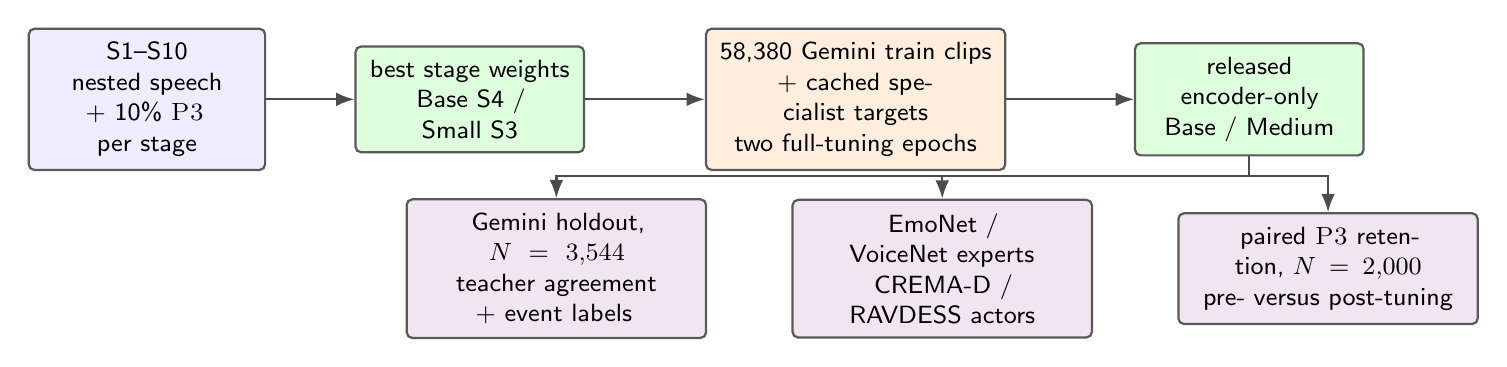
\begin{tikzpicture}[
  >=Latex, font=\sffamily\small,
  box/.style={draw=black!65,rounded corners=2pt,thick,align=center,minimum height=1.05cm,inner sep=5pt},
  data/.style={box,fill=blue!7},
  model/.style={box,fill=green!13},
  teacher/.style={box,fill=orange!13},
  test/.style={box,fill=violet!10},
  arr/.style={->,thick,draw=black!70}
]
\node[data,text width=2.65cm] (ladder) at (0,1.5) {S1--S10 nested speech\\+ 10\% \pthree\ per stage};
\node[model,text width=2.55cm] (stages) at (4.1,1.5) {best stage weights\\Base S4 / Small S3};
\node[teacher,text width=3.45cm] (adapt) at (9.0,1.5) {58,380 Gemini train clips\\+ cached specialist targets\\two full-tuning epochs};
\node[model,text width=2.55cm] (release) at (14.0,1.5) {released encoder-only\\Base / Medium};
\node[test,text width=3.45cm] (gem) at (5.2,-0.65) {Gemini holdout, $N=3{,}544$\\teacher agreement + event labels};
\node[test,text width=3.45cm] (human) at (10.1,-0.65) {EmoNet / VoiceNet experts\\CREMA-D / RAVDESS actors};
\node[test,text width=3.45cm] (p3) at (15.0,-0.65) {paired \pthree\ retention, $N=2{,}000$\\pre- versus post-tuning};
\draw[arr] (ladder)--(stages);
\draw[arr] (stages)--(adapt);
\draw[arr] (adapt)--(release);
\draw[arr] (release.south) -- ++(0,-.25) -| (gem.north);
\draw[arr] (release.south) -- ++(0,-.25) -| (human.north);
\draw[arr] (release.south) -- ++(0,-.25) -| (p3.north);
\end{tikzpicture}%
}

\caption{Training and evaluation provenance. The curriculum, Gemini adaptation, and benchmark sets answer different questions. The specialist targets on the Gemini test quantify distillation, while EmoNet/VoiceNet and acted corpora carry external human labels. The paired \pthree\ subset measures retention across adaptation on identical clips.}
\label{fig:study-flow}
\end{figure*}

\section{Evaluation Protocols}
We report four distinct questions. \emph{Teacher agreement:} on the same 3,544 Gemini test clips, normalized MAE is mean absolute error divided by each target's training standard deviation; speaker embeddings use mean cosine on 1,718 valid single-speaker clips. \emph{Human-label emotion:} on the released EmoNet-Voice snapshot, 40 of 42 queried labels map to emotion heads (12,000 pairs). Expert intensities 0/1/2 are mapped to 0/5/10; student 0--4 outputs are multiplied by 2.5 and clipped. The 687 over-30-s samples use only the first 30 s. This is not the paper's full 12,600-pair protocol \citep{schuhmann2025emonetvoice}.

\emph{VoiceNet:} VoiceNet-Emo (7,986 pairs) and VoiceNet-Ext (13,917 non-language pairs) retain items with at least two raters. The emotion adapter uses the corresponding scalar; for a queried VoiceNet ordinal level $q$, the score is $-|\hat y-q|$. We report mean per-prompt Spearman $\rho$ and distinguish per-prompt thresholds fitted on the evaluated labels (oracle ``bal@pp'') from five-fold, clip-grouped threshold transfer. The current Ext file has fewer qualifying items than the 16,166 reported in \citet{schuhmann2026voicenet}, so published VoiceCLAP numbers are context, not a controlled same-row comparison.

\emph{Acted and timed tasks:} CREMA-D (7,442 clips, 91 actors) and RAVDESS speech (1,440 clips, 24 actors) \citep{cao2014cremad,livingstone2018ravdess} use both a fixed 40-to-basic-emotion crosswalk and a supervised readout from all 192 frozen student scores. This readout standardizes scores using training-fold statistics and fits a 64-unit GELU multilayer perceptron; five actor-disjoint outer folds and three inner folds select learning rate and epochs. These adapted accuracies measure supervised transfer, not zero-shot recognition. Vocal events use frame F1 at a fixed 0.5 threshold and one-to-one event matching at interval IoU $\geq0.5$; boundary errors are conditional on matched events. We compare pre/post-Gemini checkpoints on the same \pthree\ subset. A separate 300-clip locator mixture evaluates only the \emph{pre-Gemini} S4/S3 models; its source pools might overlap \pthree. It is a mixture-domain stress test, not certified unseen-source generalization.

\section{Results}
\begin{table*}[t]
\centering\small
\caption{External human-label tests. Higher is better. The EmoNet and VoiceNet paper rows use their own full datasets or snapshots and interfaces; they are shown for orientation, not as matched-sample significance claims. Acted-corpus results use an additional nested actor-disjoint 192-score MLP adapter.}
\label{tab:external}
\resizebox{\textwidth}{!}{\begin{tabular}{@{}llcccc@{}}\toprule
Benchmark & Measure & Base & Medium & Published reference & Reference system \\\midrule
EmoNet-Voice mapped 40, $N=12{,}000$ & Pearson $r$ & 0.434 & 0.451 & 0.414 / 0.421 & Empathic Insight Small / Large$^a$ \\
VoiceNet-Emo, $N=7{,}986$ & mean prompt $\rho$ & 0.429 & 0.428 & 0.372 & VoiceCLAP-Large$^b$ \\
VoiceNet-Ext, $N=13{,}917$ & mean prompt $\rho$ & 0.157 & 0.150 & 0.148 & VoiceCLAP-Large$^b$ \\
CREMA-D, $N=7{,}442$ & actor-CV accuracy & 63.10\% & 64.23\% & --- & supervised adapter \\
RAVDESS speech, $N=1{,}440$ & actor-CV accuracy & 65.97\% & 66.39\% & --- & supervised adapter \\
\bottomrule\end{tabular}}
\vspace{2pt}\parbox{0.97\textwidth}{\footnotesize $^a$Paper uses 12,600 pairs; our 12,000-pair mapping excludes two non-emotion labels. $^b$VoiceNet Table 1 uses a different snapshot and cosine audio--text scores; its VoiceNet-Ext >=2-rater count is 16,166, versus 13,917 here. No confidence interval or paired test supports a superiority claim.}
\end{table*}

On expert-labeled EmoNet, Medium's mapped Pearson is 0.451, while Base reaches 0.434; the comparison to Empathic Insight in Table~\ref{tab:external} is descriptive because the sample set differs. VoiceNet emotion rank association is similar across sizes; Ext remains low. A fixed, no-label-fitted crosswalk produces only 18.9/19.7\% CREMA-D and 24.8/24.7\% RAVDESS top-1 accuracy. The increase from the supervised actor-disjoint readout therefore measures adaptation to each acted taxonomy, not native zero-shot categorization.

\begin{table}[t]
\centering\small
\caption{Identical held-out Gemini clips ($N=3{,}544$); lower normalized MAE, higher cosine and F1 are better. Scalars are compared with machine annotations. Speaker cosine uses $N=1{,}718$; other masks vary.}
\label{tab:teacher}
\begin{tabular}{@{}lcc@{}}\toprule
Measure & Base & Medium \\\midrule
40 emotions, mean $\nmae$ & 0.587 & 0.561 \\
57 voice dimensions, mean $\nmae$ & 0.497 & 0.481 \\
AudioBox four, mean $\nmae$ & 0.188 & 0.174 \\
DNSMOS seven, mean $\nmae$ & 0.205 & 0.198 \\
Timbre / identity cosine & .904 / .854 & .922 / .874 \\
CPS raw MAE, char/s & 0.901 & 0.931 \\
Burst frame F1 & 0.693 & 0.689 \\
Event F1, IoU $\geq0.5$ & 0.194 & 0.195 \\
Event precision / recall & .111 / .775 & .112 / .767 \\
Matched start / end MAE, s & .120 / .197 & .115 / .201 \\
True-span burst-class accuracy & 0.428 & 0.448 \\
\bottomrule\end{tabular}
\end{table}

Medium better matches the specialist quality and speaker-vector teachers, but neither size solves localization on the Gemini annotations. Giving the classifier reference intervals raises type accuracy to 0.448 at best, illustrating that class recognition and event discovery are different problems. The 192-target result set, including genuineness, blend and every quality axis, is supplied in machine-readable evidence rather than compressed into a single mean.

\begin{table}[t]
\centering\small
\caption{Before/after vocal-burst retention on the \emph{same fixed 2,000-clip} \pthree\ test subset. ``Pre'' is the selected S4/S3 checkpoint; ``post'' is the Gemini-tuned model.}
\label{tab:burst}
\begin{tabular}{@{}llcc@{}}\toprule
Model & Phase & \pthree\ frame F1 & \pthree\ event F1 \\\midrule
Base & pre & .962 & .750 \\
Base & post & .805 & .386 \\
Medium & pre & .969 & .796 \\
Medium & post & .839 & .435 \\
\bottomrule\end{tabular}
\end{table}

The evaluation distinguishes two \pthree\ protocols: a 9,693-clip pre-tune test and the fixed 2,000-clip before/after retention subset in Table~\ref{tab:burst}. On the latter, Base frame F1 drops from .962 to .805 and event F1 from .750 to .386; Medium drops from .969 to .839 and .796 to .435. On the separate locator mixture, the \emph{pre-tune} models obtain frame F1 .263/.279 and binary-region F1 .065/.063. It contains music/effect-heavy cases and was not threshold-calibrated. The final Gemini-tuned checkpoints have not been evaluated on this locator mixture. These results argue against treating synthetic-insertion success as general burst localization.

\paragraph{Backbone comparison and development history.}
In a controlled preliminary 100-target experiment, Base/S9 had validation Huber .1362 versus Tiny/S9 .1466; S10 gave .1662/.1749, with more data and updates coupled in S9. The later layered Base/Medium curriculum adds speaker and event heads. A separate CLAPv2 XS/M study uses one S8 warm-up pass and two Gemini epochs; its audio towers have 16.6M/64.4M parameters. On the same Gemini test, CLAP XS/M event F1 is .302/.299, exceeding Whisper Base/Medium .194/.195, while Whisper has much higher timbre cosine (.904/.922 versus .723/.713). On mapped EmoNet, Whisper Spearman .458/.468 exceeds CLAP .374/.391; CLAP M has stronger VoiceNet-Ext $\rho$ (.163 versus Medium .150). Differences in pretraining and warm-up prevent an architecture-only causal claim.

\section{Discussion and Limitations}
The broad output set is useful for a single-pass annotation service, but the evidence has four boundaries. First, most training labels and held-out target scores come from teachers, so high correlations measure imitation; only external human-label benchmarks test human agreement. Second, VoiceNet and EmoNet paper comparators use different snapshots, sample filters, and interfaces, and our actor-CV classifiers are supervised transfer. Third, the 30-s input limit truncates long benchmark clips, and burst probabilities are uncalibrated. Fourth, the curriculum's large synthetic \pthree\ pool and Gemini adaptation produce a visible localization transfer gap; the fixed 0.5 threshold and source uncertainty limit generalization claims. We did not run a controlled single-task-versus-multitask ablation, so the benefits of joint training over separate models remain unquantified.

The model predicts \emph{perceived} qualities and teacher-defined representations. Emotion, genuineness, and identity vectors should not be treated as diagnoses, personal attributes, or biometric identification. Large-scale web-data annotation also requires source licensing, consent, and domain-specific evaluation beyond this paper. The model can prioritize data for review; its scores should retain teacher provenance and uncertainty about people.

\section{Conclusion}
\he\ packages dense speech descriptors and timed vocal events into two fully fine-tuned, encoder-only Whisper models. External emotion tests show useful association with expert labels and held-out teacher tests show broad target coverage. The main open problem is robust interval localization across soundscape conditions; this is a concrete target for revised data mixtures, replay during adaptation, and stronger event supervision.

\section*{Impact Statement}
This work provides an audio annotation model that may help organize large speech collections. Its predictions can mischaracterize emotions or voice traits, and its speaker vectors could be misused if interpreted as identity evidence. We recommend limiting these outputs to research and curation workflows with source rights, human review for consequential uses, and explicit reporting of domain transfer performance.

\bibliography{references}
\bibliographystyle{icml2026}

\appendix
\section{Additional Reproducibility Detail}
\paragraph{Score inventory.} The 192 scalar outputs are partitioned $40+57+3+19+4+7+61+1$. The extra 19 include background quality, recording quality, overall/speech quality and content enjoyment; the AudioBox four are CE, CU, PC and PQ; the DNSMOS seven are raw and calibrated SIG/BAK/OVRL plus P808 MOS. The 61 VoiceCLAP attributes partly overlap the 40 emotions but remain separate output slots. The model never emits a VoiceCLAP intermediate embedding. The blend target is masked for no-burst clips.

\paragraph{Teacher inventory.} OpenAI Whisper Base and Small supply only the initial audio encoder weights. The recorded \texttt{gemini-3.8-flash} annotator supplies valid emotion, VoiceNet, genuineness/blend, overlapping VoiceCLAP emotion, CPS, count and event labels. Original emotion and the 19 extra targets come from Empathic Insight Voice Plus/BUD-E; original 57-style labels come from commercial VoiceNet dimension predictors. Remaining VoiceCLAP attributes, AudioBox, DNSMOS and Orange vectors retain their specialist sources. Sidecars also cache 768D VoiceCLAP and 3,072D BUD-E intermediate features, but the student does not predict them or load teachers at inference. The full ordered target schema and normalization are supplied as CSV and JSON in the bundle.

\paragraph{Checks and checkpoints.} Early S10/S9 experiments used three epochs each and a common 2,048-clip UID-disjoint validation. The layered curriculum saved a best state in each S1--S10 stage, selected on fixed Ladder plus \pthree\ validation. It retained AdamW, schedule, random states and data hashes. Gemini adaptation strictly restored Base S4 / Small S3 weights and initialized a new optimizer. Its two validation losses declined from 1.8121 to 1.7684 (Base) and 1.7446 to 1.6989 (Medium). The 53 event classes were weighted from training counts only. No MOSS caption adapter or ASR decoder is included in these weights.

\paragraph{Protocol distinctions.} \pthree\ binary-region matching merges overlapping source bursts; the proposal head can recover them separately. Frame F1 is calculated over valid 20-ms bins; event F1 uses one-to-one matching. Onset/offset errors are defined only for matched intervals and should never be read as the error of all events. The published VoiceNet paper reports per-prompt thresholded balanced accuracy, which can fit a threshold on the scored labels; the additional grouped-fold version tests threshold transfer. The EmoNet-Voice comparison excludes its two non-emotion queried labels. CREMA-D and RAVDESS nested folds group by actor; the final-model readout receives all 192 predicted scores and trains only on its training folds. An earlier, separate pre-Gemini analysis used an 80-score linear classifier and should not be conflated with these results.

\paragraph{Reproducibility assets.} The local paper bundle includes a claim/source ledger, checked bibliography, selected run configurations and metric snapshots. Full training and inference code and released weights are in the companion model repositories; data and specialist-teacher rights follow their source cards. No credentials or raw recordings are bundled with this manuscript.
\end{document}
